\PassOptionsToPackage{unicode=true}{hyperref} % options for packages loaded elsewhere
\PassOptionsToPackage{hyphens}{url}
%
\documentclass[]{article}
\usepackage{lmodern}
\usepackage{amssymb,amsmath}
\usepackage{ifxetex,ifluatex}
\usepackage{lscape}
\usepackage{graphicx}
\usepackage{float}
%    \usepackage{lscape}
\usepackage{rotating}
\usepackage{fixltx2e} % provides \textsubscript
\ifnum 0\ifxetex 1\fi\ifluatex 1\fi=0 % if pdftex
  \usepackage[T1]{fontenc}
  \usepackage[utf8]{inputenc}
  \usepackage{textcomp} % provides euro and other symbols
\else % if luatex or xelatex
  \usepackage{unicode-math}
  \defaultfontfeatures{Ligatures=TeX,Scale=MatchLowercase}
\fi
% use upquote if available, for straight quotes in verbatim environments
\IfFileExists{upquote.sty}{\usepackage{upquote}}{}
% use microtype if available
\IfFileExists{microtype.sty}{%
\usepackage[]{microtype}
\UseMicrotypeSet[protrusion]{basicmath} % disable protrusion for tt fonts
}{}
\IfFileExists{parskip.sty}{%
\usepackage{parskip}
}{% else
\setlength{\parindent}{0pt}
\setlength{\parskip}{6pt plus 2pt minus 1pt}
}
\usepackage{hyperref}
\hypersetup{
            pdftitle={arc42 Template},
            pdfborder={0 0 0},
            breaklinks=true}
\urlstyle{same}  % don't use monospace font for urls
\usepackage{longtable,booktabs}
% Fix footnotes in tables (requires footnote package)
\IfFileExists{footnote.sty}{\usepackage{footnote}\makesavenoteenv{longtable}}{}
\usepackage{graphicx,grffile}
\makeatletter
\def\maxwidth{\ifdim\Gin@nat@width>\linewidth\linewidth\else\Gin@nat@width\fi}
\def\maxheight{\ifdim\Gin@nat@height>\textheight\textheight\else\Gin@nat@height\fi}
\makeatother
% Scale images if necessary, so that they will not overflow the page
% margins by default, and it is still possible to overwrite the defaults
% using explicit options in \includegraphics[width, height, ...]{}
\setkeys{Gin}{width=\maxwidth,height=\maxheight,keepaspectratio}
\setlength{\emergencystretch}{3em}  % prevent overfull lines
\providecommand{\tightlist}{%
  \setlength{\itemsep}{0pt}\setlength{\parskip}{0pt}}
\setcounter{secnumdepth}{0}
% Redefines (sub)paragraphs to behave more like sections
\ifx\paragraph\undefined\else
\let\oldparagraph\paragraph
\renewcommand{\paragraph}[1]{\oldparagraph{#1}\mbox{}}
\fi
\ifx\subparagraph\undefined\else
\let\oldsubparagraph\subparagraph
\renewcommand{\subparagraph}[1]{\oldsubparagraph{#1}\mbox{}}
\fi

% set default figure placement to htbp
\makeatletter
\def\fps@figure{htbp}
\makeatother


\title{
\includegraphics{images/arc42-logo.png} Template}
\date{2019-01-04}

\begin{document}
\maketitle

\section{}

\textbf{Über arc42}

arc42, das Template zur Dokumentation von Software- und
Systemarchitekturen.

Erstellt von Dr. Gernot Starke, Dr. Peter Hruschka und Mitwirkenden.

Template Revision: 7.0 DE (asciidoc-based), January 2017

© We acknowledge that this document uses material from the arc42
architecture template, \url{http://www.arc42.de}. Created by Dr. Peter
Hruschka \& Dr. Gernot Starke.

\begin{quote}
\textbf{Note}

Diese Version des Templates enthält Hilfen und Erläuterungen. Sie dient
der Einarbeitung in arc42 sowie dem Verständnis der Konzepte. Für die
Dokumentation eigener System verwenden Sie besser die \emph{plain}
Version.
\end{quote}

\hypertarget{section-introduction-and-goals}{%
\section{Einführung und Ziele}\label{section-introduction-and-goals}}

Beschreibt die wesentlichen Anforderungen und treibenden Kräfte, die bei
der Umsetzung der Softwarearchitektur und Entwicklung des Systems
berücksichtigt werden müssen.

Dazu gehören:

\begin{itemize}
\item
  zugrunde liegende Geschäftsziele,
\item
  wesentliche Aufgabenstellungen und
\item
  essenzielle fachliche Anforderungen an das System sowie
\item
  Qualitätsziele für die Architektur und
\item
  relevante Stakeholder und deren Erwartungshaltung.
\end{itemize}

\hypertarget{_aufgabenstellung}{%
\subsection{Aufgabenstellung}\label{_aufgabenstellung}}

\textbf{Inhalt.}

Kurzbeschreibung der fachlichen Aufgabenstellung, treibenden Kräfte,
Extrakt (oder Abstract) der Anforderungen. Verweis auf (hoffentlich
vorliegende) Anforderungsdokumente (mit Versionsbezeichnungen und
Ablageorten).

\textbf{Motivation.}

Aus Sicht der späteren Nutzung ist die Unterstützung einer fachlichen
Aufgabe oder Verbesserung der Qualität der eigentliche Beweggrund, ein
neues System zu schaffen oder ein bestehendes zu modifizieren.

\textbf{Form.}

Kurze textuelle Beschreibung, eventuell in tabellarischer Use-Case Form.
Sofern vorhanden, sollte die Aufgabenstellung Verweise auf die
entsprechenden Anforderungsdokumente enthalten.

Halten Sie diese Auszüge so knapp wie möglich und wägen Sie Lesbarkeit
und Redundanzfreiheit gegeneinander ab.

\hypertarget{_qualit_tsziele}{%
\subsection{Qualitätsziele}\label{_qualit_tsziele}}

\textbf{Inhalt.}

Die Top-3 bis Top-5 der Qualitätsziele für die Architektur, deren
Erfüllung oder Einhaltung den maßgeblichen Stakeholdern besonders
wichtig sind. Gemeint sind hier wirklich Qualitätsziele, die nicht
unbedingt mit den Zielen des Projekts übereinstimmen. Beachten Sie den
Unterschied.

\textbf{Motivation.}

Weil Qualitätsziele grundlegende Architekturentscheidungen oft
maßgeblich beeinflussen, sollten Sie die für Ihre Stakeholder relevanten
Qualitätsziele kennen, möglichst konkret und operationalisierbar.

\textbf{Form.}

Tabellarische Darstellung der Qualitätsziele mit möglichst konkreten
Szenarien, geordnet nach Prioritäten.

\hypertarget{_stakeholder}{%
\subsection{Stakeholder}\label{_stakeholder}}

\begin{longtable}[]{@{}lll@{}}
\toprule
\begin{minipage}[b]{0.23\columnwidth}\raggedright
Rolle\strut
\end{minipage} & \begin{minipage}[b]{0.23\columnwidth}\raggedright
Kontakt\strut
\end{minipage} & \begin{minipage}[b]{0.46\columnwidth}\raggedright
Erwartungshaltung\strut
\end{minipage}\tabularnewline
\midrule
\endhead
\begin{minipage}[t]{0.23\columnwidth}\raggedright
	\emph{CEO}\strut
\end{minipage} & \begin{minipage}[t]{0.23\columnwidth}\raggedright
\emph{Dr. Michael Moore}\strut
\end{minipage} & \begin{minipage}[t]{0.46\columnwidth}\raggedright
\emph{Keine Vollautomatisierung, Segnet alle Boni manuell ab}\strut
\end{minipage}\tabularnewline
\begin{minipage}[t]{0.23\columnwidth}\raggedright
\emph{HR Senior Consultant}\strut
\end{minipage} & \begin{minipage}[t]{0.23\columnwidth}\raggedright
\emph{Chantal Banks}\strut
\end{minipage} & \begin{minipage}[t]{0.46\columnwidth}\raggedright
\emph{Weniger manuelle Schritte, Keine Papierarbeit mehr}\strut
\end{minipage}\tabularnewline
\begin{minipage}[t]{0.23\columnwidth}\raggedright
	\emph{IT-Admin}\strut
\end{minipage} & \begin{minipage}[t]{0.23\columnwidth}\raggedright
	\emph{Tom Foster}\strut
\end{minipage} & \begin{minipage}[t]{0.46\columnwidth}\raggedright
	\emph{Keine Berührungspunkte mit dem gesamten Prozess}\strut
\end{minipage}\tabularnewline
\bottomrule
\end{longtable}


\hypertarget{section-architecture-constraints}{%
\section{Randbedingungen}\label{section-architecture-constraints}}

\textbf{Inhalt.}

Beschreibung der zu nutzenden externen Systemen

\textbf{Was ist die prinzipielle Aufgabe der Anwendung OpenCRX? }
\begin{itemize}
\item CRM System
\item Account management
\item Product and Price Management
\item Sales Pipeline
\item Issue tracking
\item Groupware
\item mail, contact and calendar management
\end{itemize}

\textbf{Was ist die prinzipielle Aufgabe der Anwendung OrangeHRM? }
\begin{itemize}
	\item an Resource Management
	\item mance Management
	\item  Administration and Personal Information Management
	\item  Recruitment etc.
	\item  Employee Self Service (Time Tracking)
\end{itemize}

\textbf{Welche grundlegenden Funktionen besitzen diese Anwendungen?}
OrangeHRM bietet Funktionalitäten zum Verwalten des Personals und alles was dazu gehört:
\begin{itemize}
	\item Mitarbeiterverwaltung inkl. Mitarbeiter Self Service
	\item Dashboards
	\item Mitarbeiter Training
	\item Reiseplanung
	\item Dokumentenmanager
	\item OpenCRX bietet Funktionalitäten zur Verwaltung von Kunden
	\item Kundensupport
	\item Customer Success
	\item Marketing
	\item Analytics
	\item Sales Management
\end{itemize}

\textbf{Welche Geschäftsobjekte werden in OpenCRX bzw. OrangeHRM verwaltet?}
\begin{itemize}
	\item Kunden
	\item Mitarbeiter
\end{itemize}
\textbf{Welche Art Schnittstellen bieten OpenCRX bzw. OrangeHRM an?}
	\begin{itemize}
	\item OpenCRX:
	\begin{itemize}
		\item REST API
		\item AirSync ActiveSync
		\item User Interface (WebUI)
	\end{itemize}
	\item OrangeHRM:
		\begin{itemize}
			\item REST API
			\item Mobile APP
			\item User Interface (WebUI)
		\end{itemize}
\end{itemize}


\hypertarget{section-system-scope-and-context}{%
\section{Kontextabgrenzung}\label{section-system-scope-and-context}}
\begin{itemize}
\item
  Diverse Kontextdiagramme
\item
  Listen von Kommunikationsbeziehungen mit deren Schnittstellen
\end{itemize}

\hypertarget{_fachlicher_kontext}{%
\subsection{Fachlicher Kontext}\label{_fachlicher_kontext}}

Der Prozess kann von einem HR Senior innerhalb von der Camunda Plattform gestartet werden und beim Start wir direkt der entsprechende Mitarbeiter in das angebotene Formular-Feld eingetragen.

Weiterhin wird dem CEO ein entsprechendes Formular, in Camunda, mit einer Aufstellung der berechneten Boni zur Verfügung gestellt, in dem er Korrekturen an den einzelnen Boni vornehmen kann und entsprechend speichern, damit sie im fortlaufenden Prozess berücksichtigt werden.

\hypertarget{_technischer_kontext}{%
\subsection{Technischer Kontext}\label{_technischer_kontext}}

Die Camunda-Engine nutzt die bereitgestellte RESTful-Schnittstelle des Data-Colletors, um entsprechende Informationen über den zu bearbeitenden Salesman auszutauschen.
Hierbei wird das sogenannte ClientInfoDTO ausgetauscht.

\textbf{Data Collector - Objekte}
\begin{verbatim}
data class ClientInfoDTO(
    var salesmanName: String = "",
    var salesInfos: ArrayList<SalesInfoDTO> = ArrayList()
)

data class SalesInfoDTO(
    var productName: String = "",
    var clientName: String = "",
    var clientRanking: Int = 0,
    var quantity: Double = 0.0,
    var bonus: Int = 0
)
\end{verbatim}

Der Data-Collector kommuniziert entsprechend über RESTful Schnittstelle mit den Systemen OrangeHRM und OpenCRX, um die entsprechenden Daten zu erfassen.

\textbf{OrangeHRM - Objekte}
\begin{verbatim}
	data class Employee(
    val firstName: String,
    val lastName: String,
    val employeeId: String,
    val jobTitle: String
)

data class Organization(
    val id: String,
    val name: String,
    val email: String?,
    val country: String,
    val numberOfEmployees: String
)
\end{verbatim}

\textbf{OpenCRX - Objekte}
\begin{verbatim}
	data class Account(
    val firstName: String? = "",
    val lastName: String? = "",
    val fullName: String? = "",
    val familyStatus: Int = 0,
    val organization: String? = "",
    val jobTitle: String? = "",
    val gender: Int = 0,
    val preferredSpokenLanguage: Int = 0,
    val accountRating: Int = 0,
    val industry: String? = "",
    val annualIncomeCurrency: Int = 0,
    @JsonProperty("@href") val accountUrl: String? = ""
)
\end{verbatim}

Abbildung \ref{fig:uebung64kontextsicht} zeigt die entsprechenden Kommunikationskanäle via HTTP zwischen den technischen Systemen.

\begin{figure}[H]
	\centering
	\includegraphics[width=1.0\linewidth]{"images/uebung6_4_kontext_sicht"}
	\caption{Kontext des Systems}
	\label{fig:uebung64kontextsicht}
\end{figure}

\hypertarget{section-solution-strategy}{%
\section{Lösungsstrategie}\label{section-solution-strategy}}

\textbf{Inhalt.}

Kurzer Überblick über die grundlegenden Entscheidungen und
Lösungsansätze, die Entwurf und Implementierung des Systems prägen.
Hierzu gehören:

\begin{itemize}
\item
  Technologieentscheidungen
\item
  Entscheidungen über die Top-Level-Zerlegung des Systems,
  beispielsweise die Verwendung gesamthaft prägender Entwurfs- oder
  Architekturmuster,
\item
  Entscheidungen zur Erreichung der wichtigsten Qualitätsanforderungen
  sowie
\item
  relevante organisatorische Entscheidungen, beispielsweise für
  bestimmte Entwicklungsprozesse oder Delegation bestimmter Aufgaben an
  andere Stakeholder.
\end{itemize}

\textbf{Motivation.}

Diese wichtigen Entscheidungen bilden wesentliche „Eckpfeiler`` der
Architektur. Von ihnen hängen viele weitere Entscheidungen oder
Implementierungsregeln ab.

\textbf{Form.}

Fassen Sie die zentralen Entwurfsentscheidungen \textbf{kurz} zusammen.
Motivieren Sie, ausgehend von Aufgabenstellung, Qualitätszielen und
Randbedingungen, was Sie entschieden haben und warum Sie so entschieden
haben. Vermeiden Sie redundante Beschreibungen und verweisen Sie eher
auf weitere Ausführungen in Folgeabschnitten.

\hypertarget{section-building-block-view}{%
\section{Bausteinsicht}\label{section-building-block-view}}

\begin{figure}[ht]
	\centering
	\includegraphics[width=1.0\linewidth]{"images/uebung6_4_baustein_sicht"}
	\caption{Bausteinsicht}
	\label{fig:uebung64bausteinsicht}
\end{figure}


\hypertarget{section-runtime-view}{\section{Laufzeitsicht}\label{section-runtime-view}}
\begin{figure}[H]
	\centering
	\rotatebox{90}{\includegraphics[width=1.7\linewidth]{"images/laufzeitsicht_high_performance_bpmn"}}
	\caption{Laufzeitsicht}
	\label{fig:laufzeitsichthighperformancebpmn}
\end{figure}


\hypertarget{section-deployment-view}{%
\section{Verteilungssicht}\label{section-deployment-view}}
\begin{figure}[H]
	\centering
	\includegraphics[width=1.0\linewidth]{"images/verteilungssicht"}
	\caption{Verteilungssicht}
	\label{fig:verteilungssicht}
\end{figure}


\hypertarget{section-concepts}{%
\section{Querschnittliche Konzepte}\label{section-concepts}}

\textbf{Inhalt.}

Dieser Abschnitt beschreibt übergreifende, prinzipielle Regelungen und
Lösungsansätze, die an mehreren Stellen (=\emph{querschittlich})
relevant sind.

Solche Konzepte betreffen oft mehrere Bausteine. Dazu können vielerlei
Themen gehören, beispielsweise:

\begin{itemize}
\item
  fachliche Modelle,
\item
  eingesetzte Architektur- oder Entwurfsmuster,
\item
  Regeln für den konkreten Einsatz von Technologien,
\item
%  prinzipielle --- meist technische --- Festlegungen übergreifender Art,
\item
  Implementierungsregeln
\end{itemize}

\textbf{Motivation.}

Konzepte bilden die Grundlage für \emph{konzeptionelle Integrität}
(Konsistenz, Homogenität) der Architektur und damit eine wesentliche
Grundlage für die innere Qualität Ihrer Systeme.

Manche dieser Themen lassen sich nur schwer als Baustein in der
Architektur unterbringen (z.B. das Thema „Sicherheit``). Hier ist der
Platz im Template, wo Sie derartige Themen geschlossen behandeln können.

\textbf{Form.}

Kann vielfältig sein:

\begin{itemize}
\item
  Konzeptpapiere mit beliebiger Gliederung,
\item
  übergreifende Modelle/Szenarien mit Notationen, die Sie auch in den
  Architektursichten nutzen,
\item
  beispielhafte Implementierung speziell für technische Konzepte,
\item
  Verweise auf „übliche`` Nutzung von Standard-Frameworks
  (beispielsweise die Nutzung von Hibernate als Object/Relational
  Mapper).
\end{itemize}

\textbf{Struktur.}

Eine mögliche (nicht aber notwendige!) Untergliederung dieses
Abschnittes könnte wie folgt aussehen (wobei die Zuordnung von Themen zu
den Gruppen nicht immer eindeutig ist):

\begin{itemize}
\item
  Fachliche Konzepte
\item
  User Experience (UX)
\item
  Sicherheitskonzepte (Safety und Security)
\item
  Architektur- und Entwurfsmuster
\item
  Unter-der-Haube
\item
  Entwicklungskonzepte
\item
  Betriebskonzepte
\end{itemize}

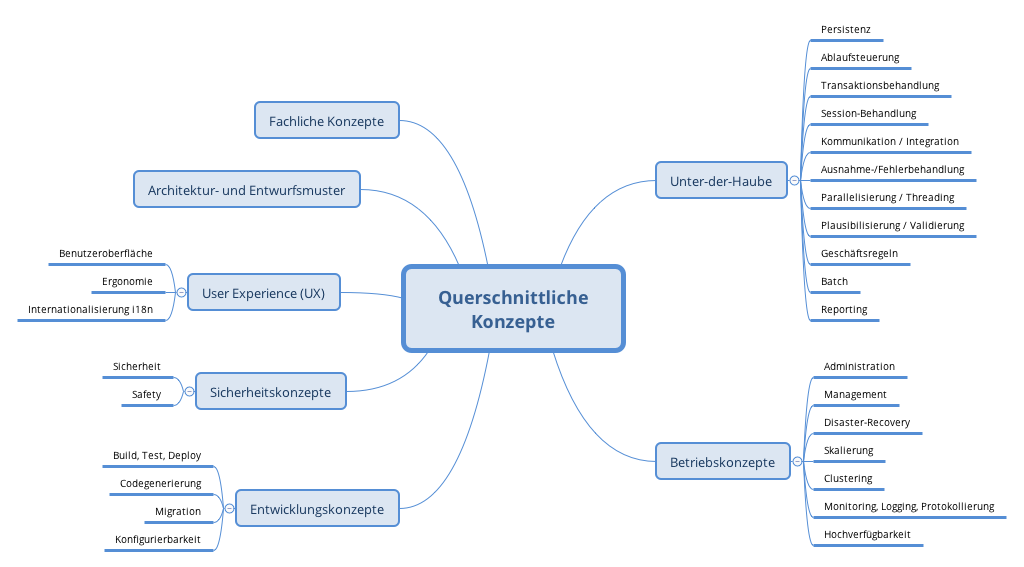
\includegraphics{images/08-Crosscutting-Concepts-Structure-DE.png}

\hypertarget{__emphasis_konzept_1_emphasis}{%
\subsection{\texorpdfstring{\emph{\textless{}Konzept
1\textgreater{}}}{\textless{}Konzept 1\textgreater{}}}\label{__emphasis_konzept_1_emphasis}}

\emph{\textless{}Erklärung\textgreater{}}

\hypertarget{__emphasis_konzept_2_emphasis}{%
\subsection{\texorpdfstring{\emph{\textless{}Konzept
2\textgreater{}}}{\textless{}Konzept 2\textgreater{}}}\label{__emphasis_konzept_2_emphasis}}

\emph{\textless{}Erklärung\textgreater{}}

\ldots{}

\hypertarget{__emphasis_konzept_n_emphasis}{%
\subsection{\texorpdfstring{\emph{\textless{}Konzept
n\textgreater{}}}{\textless{}Konzept n\textgreater{}}}\label{__emphasis_konzept_n_emphasis}}

\emph{\textless{}Erklärung\textgreater{}}

\hypertarget{section-design-decisions}{%
\section{Entwurfsentscheidungen}\label{section-design-decisions}}

Zur prototypischen Implementierung wurden verschiedene Sprachen und Technologien verwendet, welche in diesem Abschnitt erläutert werden.

Wie vorgegeben wurde zur modellierung des Workflows das Tool Camunda eingesetzt. Mithilfe von Camunda wurde der gesamte Prozess modeliert und ausgeführt. Das Camunda Cockpit und die Tasklist eignen sich hervorragend zum starten und verwalten der Prozesse. 
Da im verlaufe des Prozesses auch mit Fremdsystemen kommuniziert werden muss wurde ein Microservice in der Sprache Kotlin entwickelt. Dieser Service übernimmt die Kommunikation mit OrangeHRM und OpenCRX über die dokumentierten REST API's.
Um eine konsistene Architektur bereitzustellen bietet der Microservce ebenfalls REST-Schnittstellen an, welche aus der JavaDelegate Klasse aus Camunda heraus aufgerufen wird. 
Alle Anwendungen werden in eigenen, weitesgehend isolierten, Docker Containern betrieben.


\hypertarget{section-technical-risks}{%
\section{Risiken und technische
Schulden}\label{section-technical-risks}}

\textbf{Inhalt.}

Eine nach Prioritäten geordnete Liste der erkannten Architekturrisiken
und/oder technischen Schulden.

\begin{quote}
Risikomanagement ist Projektmanagement für Erwachsene.

---  Tim Lister Atlantic Systems Guild
\end{quote}

Unter diesem Motto sollten Sie Architekturrisiken und/oder technische
Schulden gezielt ermitteln, bewerten und Ihren Management-Stakeholdern
(z.B. Projektleitung, Product-Owner) transparent machen.

\textbf{Form.}

Liste oder Tabelle von Risiken und/oder technischen Schulden, eventuell
mit vorgeschlagenen Maßnahmen zur Risikovermeidung, Risikominimierung
oder dem Abbau der technischen Schulden.

\hypertarget{section-glossary}{%
\section{Glossar}\label{section-glossary}}

\textbf{Inhalt.}

Die wesentlichen fachlichen und technischen Begriffe, die Stakeholder im
Zusammenhang mit dem System verwenden.

Nutzen Sie das Glossar ebenfalls als Übersetzungsreferenz, falls Sie in
mehrsprachigen Teams arbeiten.

\textbf{Motivation.}

Sie sollten relevante Begriffe klar definieren, so dass alle Beteiligten

\begin{enumerate}
\def\labelenumi{\arabic{enumi}.}
\item
  diese Begriffe identisch verstehen, und
\item
  vermeiden, mehrere Begriffe für die gleiche Sache zu haben.
\end{enumerate}

\begin{itemize}
\item
  Zweispaltige Tabelle mit \textless{}Begriff\textgreater{} und
  \textless{}Definition\textgreater{}
\item
  Eventuell weitere Spalten mit Übersetzungen, falls notwendig.
\end{itemize}

\begin{longtable}[]{@{}ll@{}}
\toprule
\begin{minipage}[b]{0.31\columnwidth}\raggedright
Begriff\strut
\end{minipage} & \begin{minipage}[b]{0.63\columnwidth}\raggedright
Definition\strut
\end{minipage}\tabularnewline
\midrule
\endhead
\begin{minipage}[t]{0.31\columnwidth}\raggedright
\emph{\textless{}Begriff-1\textgreater{}}\strut
\end{minipage} & \begin{minipage}[t]{0.63\columnwidth}\raggedright
\emph{\textless{}Definition-1\textgreater{}}\strut
\end{minipage}\tabularnewline
\begin{minipage}[t]{0.31\columnwidth}\raggedright
\emph{\textless{}Begriff-2}\strut
\end{minipage} & \begin{minipage}[t]{0.63\columnwidth}\raggedright
\emph{\textless{}Definition-2\textgreater{}}\strut
\end{minipage}\tabularnewline
\bottomrule
\end{longtable}

\end{document}
